\documentclass[12pt]{article}
\usepackage{lingmacros}
\usepackage{tree-dvips}
\usepackage{enumitem}
\usepackage{cite}
\usepackage{graphicx}
\usepackage{float}
\usepackage{caption}
\begin{document}

\section*{Cu Exchange and Siting Preference in Zeolites: the Influence of the framework topology}

Zhenghang Zhao\textsuperscript{1} ..... William F. Schneider\textsuperscript{1,*}

{\small
\enumsentence{Department of Chemcial and Biomolecular Engineering, University of Notre Dame, Notre Dame, IN, 46556}
* Corresponding Author: wschnei1@nd.edu 
}                     
 
\subsection*{Abstract}

Cu-exchange SSZ-13 has been confirmed active for the selective catalytic reduction (SCR) of NO\textsubscript{X} with NH\textsubscript{3} in diesel engine aftertreatment system. The nature of the Cu siting in the SSZ-13 is essential to the redox cycle and the Cu pairability. However, SSZ-13 is a zeolite material with Chabazite topology, which contains only one symmetry-distinct tetrahedral-site and 3-dimensional pore openings. The influence of the zeolite topology in the Cu exchange is still unclear. In this work, we performed Plane-wave-based Density Functional Theory supercell calculations to investigate the Cu exchange and siting preference in 4 different frameworks. We choose FER, AEI and TON to be compared with CHA to address different features of the framework topology including the pore dimensionality, the number of distinct T-site, the double-six-ring building unit, etc. Our results show the similarity and difference between zeolite frameworks

\subsection*{Introduction}
\subsubsection*{Objectives}
We compare the types of Cu sites and exchange energetics, compositional phase diagrms among CHA, AEI, FER and TON in order to 1) understand the influence of zeolite topology, similarities and differences between different framework. 2) Propose a design strategy to guide the choice of zeolite framework to achieve specific catalytic purposes.

\subsubsection*{Justification}
\begin{enumerate}
\item Cu SSZ-13 is a ion-exchange zeolite material that has a chabazite framework. implemented as the on-board selective catalytic reduction (SCR) catalysts in diesel engine aftertreatment system. The whole SCR cycle include the pairing and oxidation of 2 Cu\textsuperscript{+} clusters to a Cu\textsuperscript{2+} oxo cluster, and the reduction of the Cu\textsuperscript{2+} back to Cu\textsuperscript{+}. Thus, the nature of the Cu$^{+}$ and Cu$^{2+}$ are essential to learn the relation between the SCR mechanism and the framework topology, Si/Al ratio, etc.
\end{enumerate}

\begin{enumerate}
\item In SSZ-13 it is now well established that Cu2+ exchanges into the framework at proximal pairs of charge-compensating framework Al within a six-membered ring (6MR) to create Z2Cu sites and at isolated framework Al to form ZCu$_{2+}$OH sites.\cite{Paolucci2016}  Experiments and calculations are consistent with preferential population of the former sites before the latter. By combining this insight with models for the distribution of Al on the SSZ-13 framework, it is possible to create a composition phase diagram for relative fractions of Z2Cu and ZCuOH in SSZ-13.\cite{Paolucci2016}
\end{enumerate}

\begin{enumerate}
\item Construction of the composition phase diagram for SSZ-13 is facilitated by the high symmetry of the CHA lattice, resulting in only one symmetry-distinct tetrahedral site. In this work, we explore extending this  methodology to lower symmetry frameworks, with a particular emphasis on AEI, FER and TON, chosen because they represent different numbers of symmetry-distinct T-site, different pore dimensionality, different building units.
\end{enumerate}

\subsubsection*{Background}
\begin{enumerate}
\item SSZ-13 is on-board catalyst for SCR
\end{enumerate}
Zeolite, a type of mesoporous aluminosilicate materials, are mainly used as catalyst in petrolieum engineering or oil refining reactions. Cu-exchange SSZ-13
 
\begin{enumerate}[resume]
\item The Cu exchange and siting have been investigated both experimentally and theoretically
\end{enumerate}

\begin{enumerate}[resume]
\item Other emerging frameworks for SCR, and the uncertainty of the zeolite topology
\end{enumerate}

\begin{enumerate}[resume]
\item Our approach in this paper
\end{enumerate}

\begin{enumerate}[resume]
\item What's new in this work
\end{enumerate}

\subsection*{Computational Methods}

CHA, FER, AEI and TON conventional unit cells were determined from the IZA structure. A 1 $\times$ 1 $\times$ 1 supercell was constructed for CHA, FER and AEI, while a 1$\times$ 1$\times$ 2 supercell was constructed for TON. For each framework, Si was  substituted by Al to cover all available T-sites. H, Cu and CuOH were placed in all possible locations in each T-site for each framework. A enumeration code was established to enumerate all possible T-site pairs for each framework, and 2 Si were substituted by Al. DFT simulations were performed using the Vienna ab-initio Simulation Package (VASP). Spin-polarized DFT energies were determined within the generalized gradient approximation and projector-augmented wave description of core states. Calculations are conducted with a 72 T-site supercell. Construction of relative energy diagrams followed the previous procedures \cite{Paolucci2016} and was further normalized to mole of exchanged Cu ions.



\subsection*{Guidance to the reader}
Here, we compute the DFT exchange energies for Z$_{2}$Cu and ZCuOH in CHA, AEI, FER and TON. We build a linear model to .....

\subsection*{Results and Disscussions}
\subsubsection*{Sites in CHA, AEI, FER and TON}
\begin{figure}[H]
\centering
 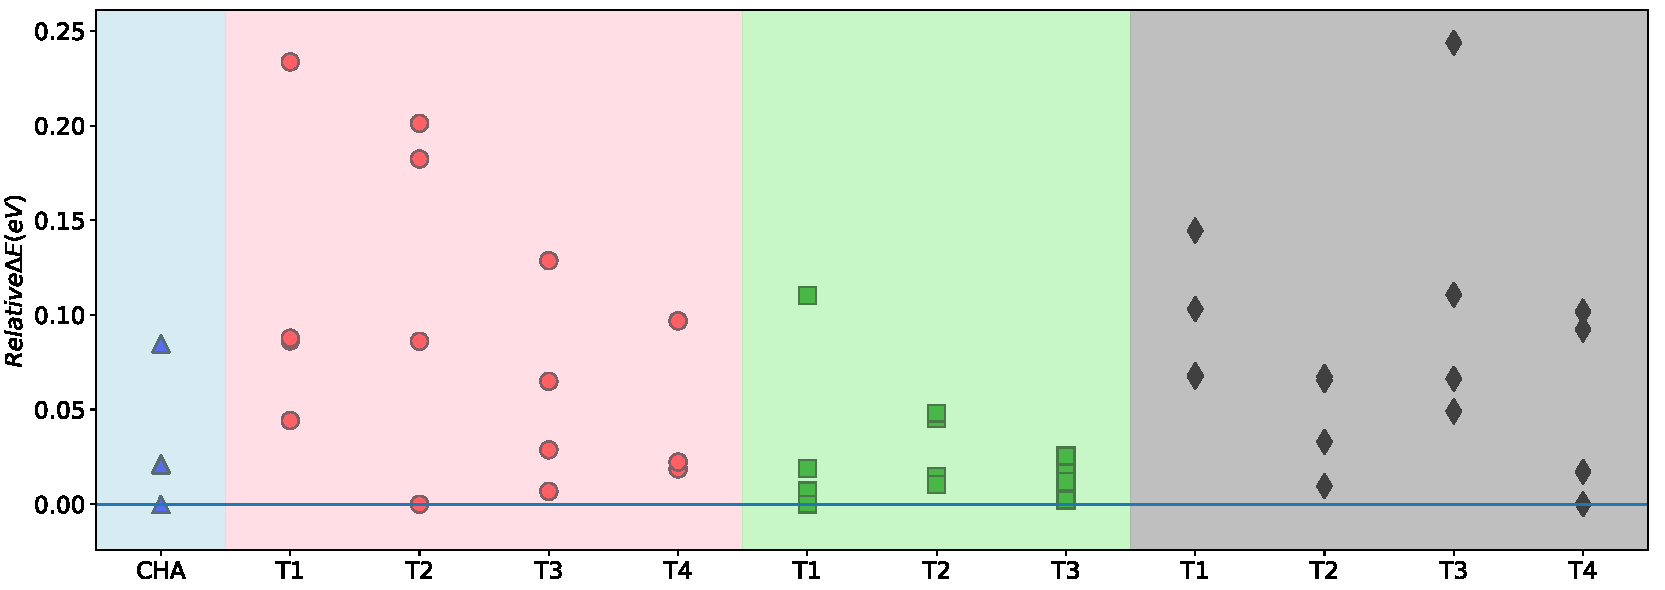
\includegraphics[width=5.2in]{./Figures/Figure-1}
 \caption{Zeolite topologies for CHA, AEI, FER and TON}
 \label{Topologies}
\end{figure}

\begin{enumerate}
\item CHA and AEI have three-dimensional window structure formed from 8-membered-ring, but a different stacking of the double 6-ring building units(Figure 1a, 1b). The resulting cages for CHA and AEI have oblate and pear-shaped cavities. FER has a two-dimensional window structure formed from both 10- and 8-membered-ring channels (Figure 1c), and TON has a one-dimensional window structure formed from 10-membered-ring channels (Figure 1d).  The consequence of different dimensional window structure is some isolated or paired Al sites are blocked by small-number-ring walls to electrostatically tether Cu ions.
\end{enumerate}

\begin{enumerate}[resume]
\item CHA has only one symmetry-distinct tetrahedral-site (T-site) (Figure 1a), while AEI has 3 symmetry-distinct T-sites (Figure 1b). Both FER and TON have 4 symmetry-distinct T-sites (Figure 1c, 1d). The numbering of different T sites are also labeled in Figure 1. Those 3 types of T-sites in AEI all have a multiplicitiy of 16 in a 48 T-site conventional AEI unit cell. T1, T2, T3 and T4 sites in FER have multiplicities of 16, 8, 8 and 4 in a 36 T-site conventional unit cell. TON has multiplicities of 8, 8, 4 and 4 for T1 to T4 sites in a 24 T-site conventional unit cell. The T4 site in TON is inaccessible to the large 10-membered-ring pore openings, resulting in different Cu ion exchange properties.
\end{enumerate}

\begin{enumerate}[resume]
\item When Cu is exchanged in the framework, it maintains either +1 or +2 state, which resulting in ZCu, ZCuOH and Z$_{2}$Cu forms. Here, Z indicates a frameworked Al site. These sites form in exchange with the bronsted-acid sites (ZH and Z$_{2}$H$_{2}$) that are pre-existed in the framework.
\end{enumerate}

\begin{enumerate}[resume]
\item The types of isolated proton and isolated Cu energies are the same to the types of symmetry-distinct T-sites in all zeolite frameworks. For the types of Z$_{2}$H$_{2}$ and Z$_{2}$Cu sites, we used a previously developed enumeration code to identify the Al proximity in 4 zeolite frameworks.\cite{Paolucci2016} The unique Al pairs are classified as "clusters" in the enumeration code, and the identified unique Al clusters, which will be included in subsequent paired Al exchange energy analysis.
\end{enumerate}



\subsubsection*{Isolated Al exchange energies}
\begin{figure}[H]
\centering
  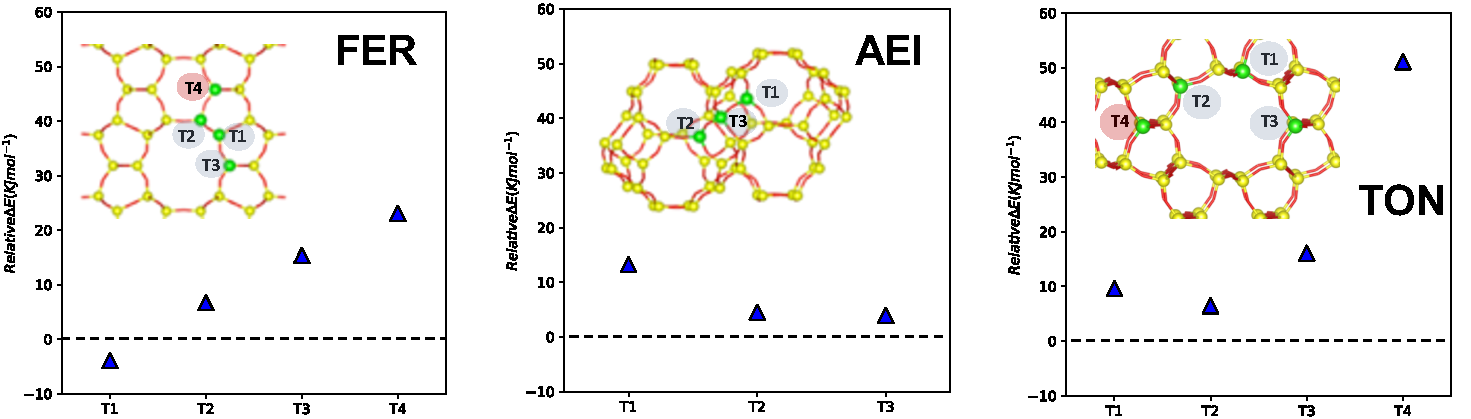
\includegraphics[width=5.2in]{./Figures/Figure-2}
  \caption{ZH exchange energies for CHA, AEI, FER and TON. Energies are normalized to the lowest energy for each T site.}
  \label{ZH energies}
\end{figure}

\begin{enumerate}
\item We picked up each framework, placed proton close to all possible 4 neighboring oxygen atoms for each T-site, and did DFT optimizations. In Figure 2, the DFT energies of ZH for all symmetry-distinct T-sites in CHA, AEI, FER and TON are plotted relative to the lowest energy for each T-site in each framework. We The optimized structures of some particular interesting points are also plotted as inserted.
\end{enumerate}

\begin{enumerate}[resume]
\item For both CHA and AEI, The energies for 4 ZH locations in each T-site are comparable to one another. All proton are pointing into the nearby large 8MR pore openings. The exceptions that draws our attention is the forth one in CHA and AEI T1. 
\end{enumerate}

\subsubsection*{ZCuOH relative to CHA}
\begin{figure}[H]
\centering
  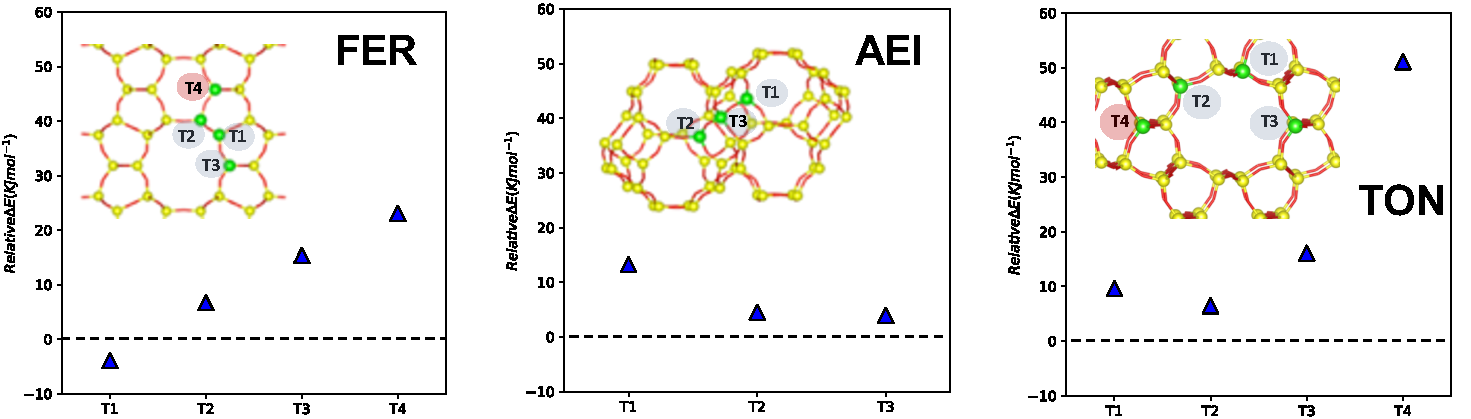
\includegraphics[width=5.2in]{./Figures/Figure-3}
  \caption{Relative ZCuOH exchange energies  for (), (), () compared to CHA.}
  \label{ZH}
\end{figure}

\subsubsection*{Z2Cu relative to CHA}
\begin{figure}[H]
\centering
  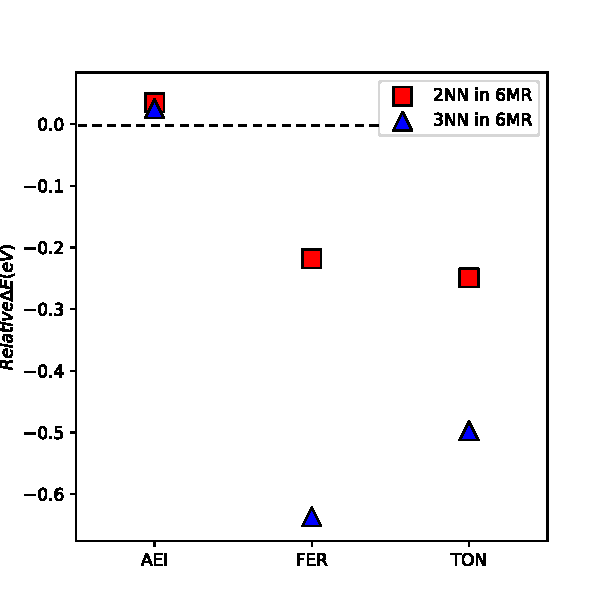
\includegraphics[width=2.6in]{./Figures/Figure-4}
  \caption{Z2Cu exchange energies relative to CHA for (), (), (), ()}
  \label{PhaseDiagram}
\end{figure}

\subsubsection*{Z2Cu to ZCuOH}



\subsubsection*{Compositional phase diagram}
\begin{figure}[H]
\centering
  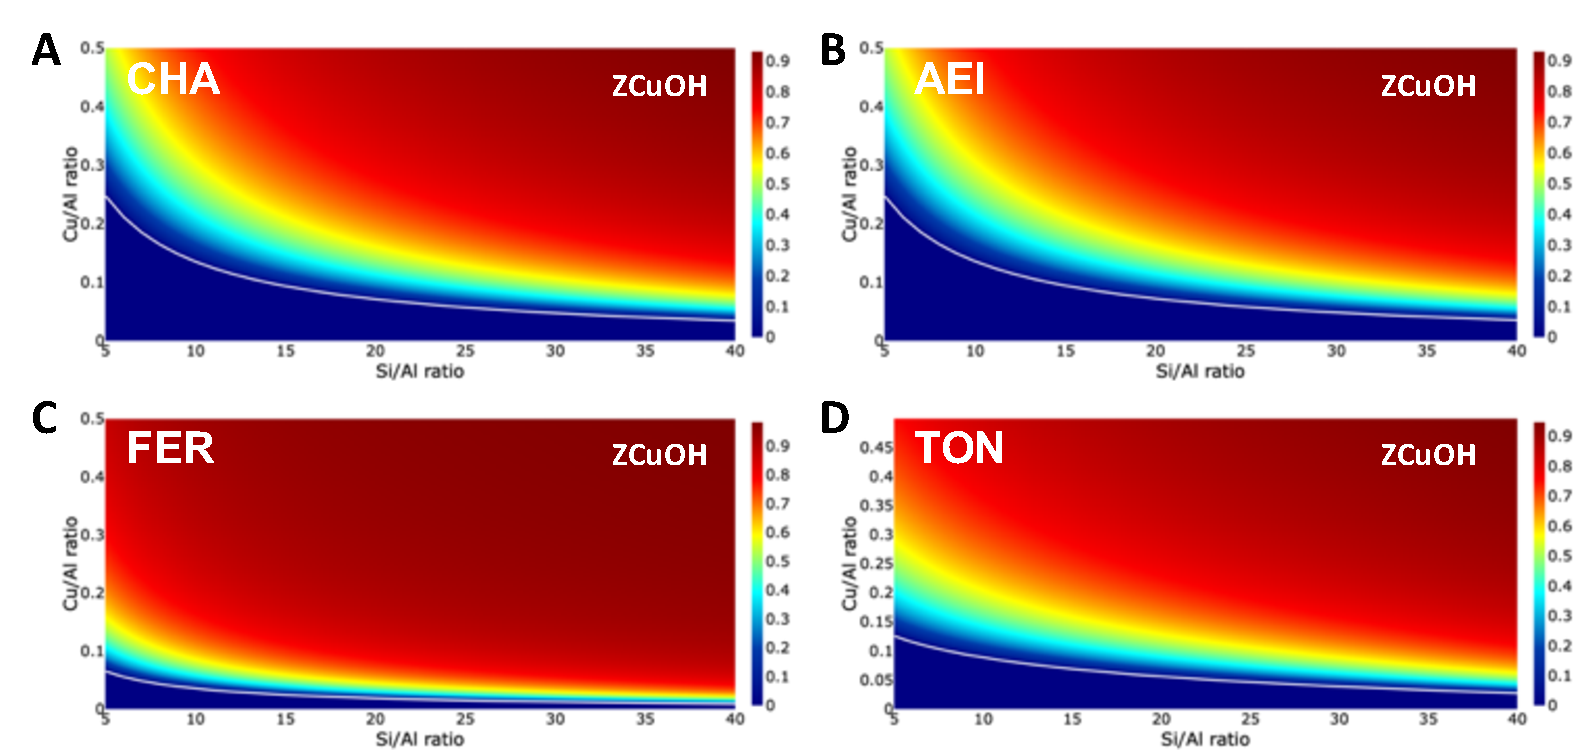
\includegraphics[width=5.2in]{./Figures/Figure-5}
  \caption{Compositional phase diagrams for (), (), (), ()}
  \label{PhaseDiagram}
\end{figure}

\subsubsection*{Fitting models}

\subsection*{Conclusions}

In this work, we interrogate and compare Cu ion exchange and siting preference in CHA, AEI, FER and TON zeolites through DFT supercell simulation, and identify the sensitivity of the  Cu$_{+}$ and Cu$_{2+}$ to the zeolite topology, which promises the potential of rational choice of zeolite topology to tailor the Cu siting  during SCR cycle. This work can be extended to predict the Cu siting of all 237 zeolite topologies for specific Cu ion properties of interest. 

\bibliographystyle{plain}
\bibliography{Cu-citing-outline}



\end{document}
